\documentclass{article}
\usepackage[left=3cm,top=3cm,right=2cm,bottom=2cm]{geometry}
\usepackage{amssymb}
\usepackage{amsmath}
\usepackage{cancel}
\usepackage{graphicx}

\title{(Universidade de São Paulo)\\
Lista 1}

\author{Cálculo II\\
Docente: Zani\\
Vinícius de Sá Ferreira -- 15491650}

\newcommand{\n}{\phantom{}}
\renewcommand{\d}[1]{\displaystyle{#1}}

\date{12 ago. 2024}

\begin{document}
    \maketitle
    
    \subsection*{1. Determine o domínio de $f$ e faça seu esboço nos seguintes casos:}
        \hspace*{12px}
        a) $\d{ f(x, y) = \frac{xy}{x - 2y} }$

        \[x - 2y \neq 0\]
        \[x \neq 2y\]
        \[\therefore dom(f) = \{(x,y) \in \mathbb{R}^2; x \neq 2y\}\]

        \[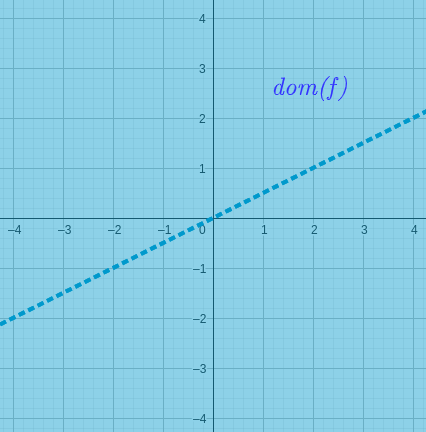
\includegraphics[width=110px]{imgs/001.png}\]

        \n

        b) $\d{ f(u, v) = \sqrt{1 - u} - e^{\frac{u}{v}} }$

        \[v \neq 0\]

        \[1 - u \geq 0\]
        \[u \geq 1\]
        \[\therefore dom(f) = \{(u,v) \in \mathbb{R}^2; u \geq 1 \textrm{ e } v \neq 0\}\]

        \[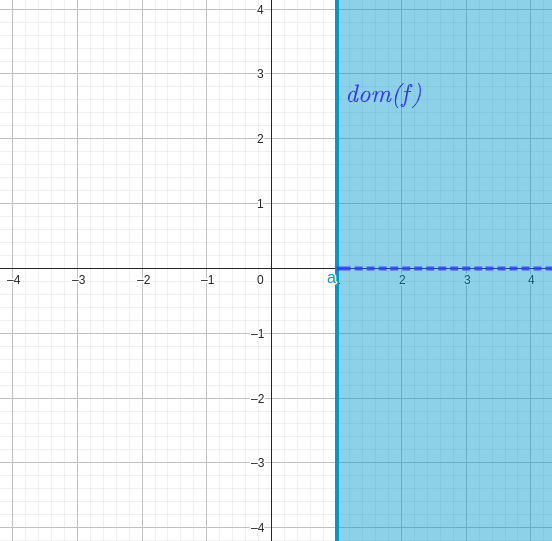
\includegraphics[width=110px]{imgs/002.png}\]

        \newpage

        c) $\d{ f(x, y) = \frac{xy}{x^2 - y^3} }$

        \[x^2 - y^3 \neq 0\]
        \[x^2 \neq y^3\]
        \[y \neq \sqrt[3]{x^2}\]
        \[\therefore dom(f) = \{(x,y) \in \mathbb{R}^2; y \neq \sqrt[3]{x^2}\}\]

        \[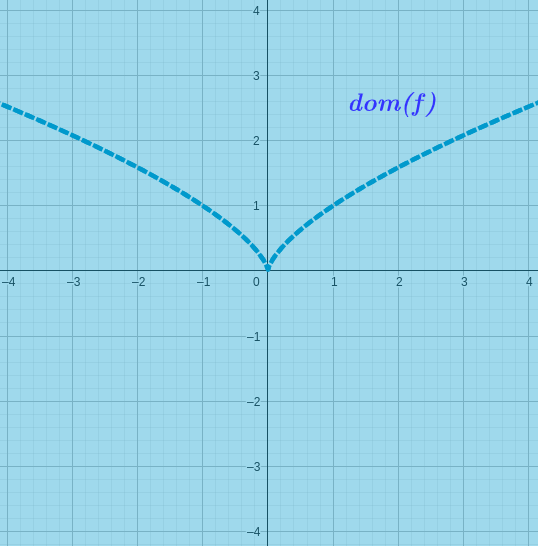
\includegraphics[width=110px]{imgs/003.png}\]

    \subsection*{2. Descreva o domínio máximo possível da função $z = f(x, y)$ dada por:}
        \hspace*{12px}
        (a) $\d{ x + y - 1 + z^2 = 0, \quad z \geq 0 }$

        \[\Leftrightarrow z = \sqrt{1 - x - y}\]
        \[1 - x - y \geq 0\]
        \[x + y \leq 1 (*)\]
        \[y \leq -x + 1\]

        \[\fbox{ $\d{ \therefore dom(z) = \{(x,y) \in \mathbb{R}^2; x + y \leq 1\} }$ }\]

        $(*)$ Reta $y = -x + 1$ e o semiplano determinado inferiormente por ela.

        \n

        (b) $\d{ z = \frac{x - y}{\sqrt{1 - x^2 - y^2}} }$

        \[\sqrt{1 - x^2 - y^2} > 0 \Leftrightarrow 1 - x^2 - y^2 > 0\]
        \[x^2 + y^2 < 1 (*)\]

        \[\fbox{ $\d{ \therefore dom(z) = \{(x,y) \in \mathbb{R}^2; x^2 + y^2 < 1\} }$ }\]

        $(*)$ Bola aberta centrada em (0,0) de raio 1.

        \n

        (c) $\d{ z = \ln(2x^2 + y^2 - 1) }$

        \[2x^2 + y^2 - 1 > 0\]
        \[2x^2 + y^2 > 1\]
        \[\frac{x^2}{\left(\frac{1}{\sqrt{2}}\right)^2} + \frac{y^2}{1^2} > 1 (*)\]

        \[\fbox{ $\d{ \therefore dom(z) = \{(x,y) \in \mathbb{R}^2; 2x^2 + y^2 > 1\} }$ }\]

        $(*)$ Complementar da elipse centrada em (0,0) de semieixos $\frac{1}{\sqrt{2}}$ e $1$.

        \newpage

        (d) $\d{ z^2 + 4 = x^2 + y^2, \quad z \geq 0 }$

        \[z^2 = x^2 + y^2 - 4\]
        \[z = \sqrt{x^2 + y^2 - 4}\]
        \[x^2 + y^2 - 4 \geq 0\]
        \[x^2 + y^2 \geq 4\]
        \[x^2 + y^2 \geq 2^2 (*)\]

        \[\fbox{ $\d{ \therefore dom(z) = \{(x,y) \in \mathbb{R}^2; x^2 + y ^2 \geq 4\} }$ }\]

        $(*)$ Complementar da bola aberta centrada em (0,0) de raio 2.

        \n

        (e) $\d{ z = \sqrt{|x| - |y|} }$

        \[|x| - |y| \geq 0\]
        \[|x| \geq |y| (*)\]

        \[\fbox{ $\d{ \therefore dom(z) = \{(x,y) \in \mathbb{R}^2; |x| \geq |y|\} }$ }\]

        $(*)$ 1º e 3º quadrantes determinado pelo sistema de coordenadas $(u,v)$ com $u: y = -x$ e $v: y = x$.

        \n

        (f) $\d{ 4x^2 + y^2 + z^2 = 1, \quad z \leq 0 }$

        \[z^2 = 1 - 4x^2 - y^2\]
        \[z = -\sqrt{1 - 4x^2 - y^2}\]
        \[1 - 4x^2 - y^2 \geq 0\]
        \[4x^2 + y^2 \leq 1\]
        \[\frac{x^2}{\left( \frac{1}{2} \right)^2} + \frac{y^2}{1^2} \leq 1 (*)\]

        \[\fbox{ $\d{ \therefore dom(z) = \{(x,y) \in \mathbb{R}^2; 4x^2 + y^2 \leq 1\} }$ }\]

        $(*)$ Elipse centrada em (0,0) de semieixos $\frac{1}{2}$ e 1 e seu interior.

        \n

    \subsection*{3. Seja $f(x, y) = x^2 + 2xy$.}
        \hspace*{12px}
        (a) Encontre as curvas de nível $c$ da função $f$, para $c = 0$ e $c \neq 0$.

        Suponha que $x = 0$, então $f$ é função constante igual a $0$. Caso contrário, suponha $x \neq 0$, então

        \[x^2 + 2xy = c\]
        \[x(x + 2y) = c\]
        \[x + 2y = \frac{c}{x}\]
        \[y = \frac{1}{2} \left(\frac{c}{x} - x\right)\]
        \[y = \frac{c-x^2}{2x}\]

        Para $c = 0$:
        \[y = -\frac{x^2}{2x} = -\frac{x}{2}\]

        (b) Encontre a interseção do gráfico de $f$ com o plano $y = mx$, $m \in \mathbb{R}$. Esboce essas curvas.

        (c) Faça um esboço do gráfico de $f$.

    \subsection*{4. Determine o domínio máximo de definição e faça um esboço das curvas de nível das funções abaixo.}
        \hspace*{12px}
        a) $f(x, y) = x - y$

        b) $f(x, y) = e^{x^2y}$

        c) $f(x, y) = \sqrt{x^2 + \frac{y^2}{4}}$

        d) $f(x, y) = \sqrt{x + y}$

        e) $f(x, y) = x^2 + y^2$

        f) $f(x, y) = \frac{1}{x^2 + y^2}$

        g) $f(x, y) = 1 - x^2 - y^2$

        h) $f(x, y) = x + y + 1$

        i) $f(x, y) = \sqrt{1 - x^2 - y^2}$

        j) $f(x, y) = x^2$, $-1 \leq x \leq 0$ e $y \geq 0$

        k) $f(x, y) = 1 - x^2$, $x \geq 0$, $y \geq 0$ e $x + y \leq 1$

        l) $f(x, y) = xy$

    \subsection*{5. Faça um esboço das superfícies de nível das funções abaixo nos níveis indicados.}
        \hspace*{12px}
        a) $f(x, y, z) = x$, $c = 1$

        b) $f(x, y, z) = y$, $c = 1$

        c) $f(x, y, z) = x^2 + y^2$, $c = 1$

        d) $f(x, y, z) = x^2 + 4y^2 + z^2$, $c = 1$

        e) $f(x, y, z) = x - y$, $c = 0, 1, 2$

        f) $f(x, y, z) = \sqrt{x^2 + \frac{y^2}{4} + \frac{z^2}{9}}$, $c = 0, 1, 2$

        g) $f(x, y, z) = \sqrt{x^2 + y^2 + z^2}$, $c = -1, 0, 2$

        h) $f(x, y, z) = xy$, $c = 0, 1, 2$

    \subsection*{6. Desenhe o traço de cada curva abaixo.}
        \hspace*{12px}
        (a) $\gamma(t) = (1, t, 1)$, $t \in \mathbb{R}$

        (b) $\gamma(t) = (1, 1, t)$, $t \geq 0$

        (c) $\gamma(t) = (t, t, 1)$, $t \geq 0$

        (d) $\gamma(t) = (\cos t, \sin t, 2)$

        (e) $\gamma(t) = (t, t, 1 + \sin t)$, $t \geq 0$

        (f) $\gamma(t) = \left(1, 1, \frac{1}{t}\right)$, $t > 0$

        (g) $\gamma(t) = (\cos t, \sin t, e^{-t})$, $t \geq 0$

        (h) $\gamma(t) = (1 + \sin t, 1 + \sin t, \cos t)$, $-\frac{\pi}{2} \leq t \leq \frac{\pi}{2}$

        (i) $\gamma(t) = (e^t \cos t, e^t \sin t)$, $t \geq 0$

    \subsection*{7. Mostre que a interseção de dois conjuntos abertos é um conjunto aberto. Mostre também que a reunião de dois conjuntos fechados é um conjunto fechado.}

    \subsection*{8. Mostre que o conjunto $A = \{(x, y) \in \mathbb{R}^2; \max\{|x|, |y|\} < 1\}$ é aberto.}

    \subsection*{9. Mostre que a fronteira da bola aberta $B(x_0, r)$ é a esfera $S(x, r) = \{x \in \mathbb{R}^n; \|x\| = r\}$.}

    \subsection*{10. O conjunto dos pontos de aderência de um conjunto também é chamado de fecho deste conjunto. Qual é o fecho de $Q_n$, isto é, qual é o conjunto $Q_n$?}

    \subsection*{11. Quais são os pontos interiores a $Q_n$, isto é, qual é o conjunto $Q_n'$?}

    \subsection*{12. Determinar o valor dos seguintes limites, caso existam:}
        \hspace*{12px}
        a) $\lim_{(x,y)\to(0,0)} e^{-1/(x^2+y^2)}$

        b) $\lim_{(x,y)\to(0,0)} \frac{x^2 - y^2}{1 + x^2 + y^2}$

        c) $\lim_{(x,y)\to(0,0)} \frac{x}{x^2 + y^2}$

        d) $\lim_{(x,y)\to(0,0)} x^2 \sin\left(\frac{y}{x}\right)$

        e) $\lim_{(x,y)\to(0,0)} (x^2 + y^2)\sin\left(\frac{1}{xy}\right)$

        f) $\lim_{(x,y)\to(0,0)} \frac{x^2y^2}{x^2y^2 + (x - y)^2}$

        g) $\lim_{(x,y)\to(0,0)} \frac{1 + x - y}{x^2 + y^2}$

        h) $\lim_{(x,y)\to(0,0)} \frac{(1 + y^2)\sin x}{x}$

        i) $\lim_{(x,y,z)\to(0,0,0)} \frac{4x - y - 3z}{2x - 5y + 2z}$

        j) $\lim_{(x,y)\to(0,0)} \frac{x^2y}{x^4 + y^2}$

        k) $\lim_{(x,y)\to(0,0)} (x^3 + 2x^2y - y^2 + 2)$

        l) $\lim_{(x,y)\to(0,0)} \frac{e^x + e^y}{\cos x + \sin y}$

        m) $\lim_{(x,y)\to(0,0)} \frac{xy}{\sqrt{x^2 + y^2}}$

        n) $\lim_{(x,y)\to(0,0)} \frac{x^4 + 3x^2y^2 + 2xy^3}{(x^2 + y^2)^2}$

        o) $\lim_{(x,y)\to(0,0)} \frac{x^2y^2}{|x| + |y|}$

        p) $\lim_{(x,y)\to(0,0)} \frac{1 + x^2y^2}{x^2 + y^2}$

        q) $\lim_{(x,y)\to(0,0)} \frac{x^2y^2}{x^4 + y^4}$

    \subsection*{13. Calcule}
    \[
        \lim_{(h,k) \to (0,0)} \frac{f(x + h, y + k) - f(x, y) - 2xh - k}{\sqrt{h^2 + k^2}}, \text{ sendo } f(x, y) = x^2 + y.
    \]

    \subsection*{14. Calcule, caso exista}
    \[
        \lim_{(h,k) \to (0,0)} \frac{f(h, k)}{\|(h, k)\|}, \text{ sendo f dada por } f(x, y) = \frac{x^3}{x^2 + y^2} \text{ e } \|(h, k)\| = \sqrt{h^2 + k^2}.
    \]

\end{document}